\documentclass[9pt,twocolumn,twoside]{article}
% Use the lineno option to display guide line numbers if required.
% Note that the use of elements such as single-column equations
% may affect the guide line number alignment.

\usepackage{amsmath}
\usepackage{graphicx}
\usepackage{subcaption}
\usepackage{breqn}
\usepackage{color}
\usepackage{subcaption}

\newcommand\davidsays[1]{{\em\color{blue} {\bf DR:} #1}}
\newcommand\forjin[1]{{\em\color{green} {\bf Jin:} #1}}
\newcommand\todo[1]{{\em\color{red} #1}}

% the follow ing causes latex to not wait interactively
% \nonstopmode

\captionsetup[subfigure]{singlelinecheck=off,justification=raggedright, margin=0pt, parskip=0pt, skip=0pt}

\title{Brownian dynamics simulation of cytoplasmic dynein's powerstroke reproduces bidirectional stepping}

\input{../../data/paper_params.tex}

\begin{document}
\maketitle

\begin{abstract}
  Please provide an abstract of no more than 250 words in a single paragraph. Abstracts should explain to the general reader the major contributions of the article. References in the abstract must be cited in full within the abstract itself and cited in the text.
\end{abstract}

\section*{TODO August 2020}
\begin{enumerate}
  \item Articulate data we fit to
  \begin{enumerate}
    \item Velocity -$\>$ unbinding rate
    \item Ratio of leading vs trailing steps -> exponential parameter
    \item Average step length -> other parameters
    \item Yildiz weird slope -> sticky rate + binding rate
    \item Avoid instant rebinds -> sticky rate
    \item Time to kick from MD??
    \item efficiency (affects instant rebind)
  \end{enumerate}
  \item Do the fit (requires 1 above)
  \paragraph{Advantages of sticky rate}
  \begin{enumerate}
    \item Accurately reflects the dynamics of a chemical process
  \end{enumerate}
\end{enumerate}

\section*{TODO January 2022}
\begin{enumerate}
\item go through and fill in missing citations
\item add more paper citations to Discussion, should tie in with more recent science. There are plenty of good uncited papers in the bibtex (10+)  
\item go through model papers and make sure none of them handle correlated stepping, since this is an impt claim we make in the intro
\item heavily edit to make it sound better, probably pretty bad right now
  \item meet with David at some point to see what he thinks
\end{enumerate}

\section*{Notes}
\begin{enumerate}
\item In my head the journal target would be Biophysical Journal; they're pretty open to modeling papers and dynein and one of the dynein modeling papers we cite was published there
\end{enumerate}

\section*{DR}
\davidsays{Fig. \ref{fig:ProbLagPlot} gives us the exponential unbinding constant. Also rerun to get better.
Explain that the bothbound time does not vary by more than X\% regardless of initial $L$ in our model.}

\davidsays{Do not add average both-bound time vs. L? This is a measurable prediction if we can't find an experimental result.  Otherwise, we can compare with experiment.  Maybe just add a sentence or two}

\davidsays{one-bound time plot. Cut?}


\newpage

%% \dropcap{C}ytoplasmic dynein-1 is a motor protein used to generate directed force in cells. The protein is a homodimer which binds to cellular filaments known as microtubules (MTs). Each monomer has several ATPase domains arranged in a larger globular domain known as the ``head''. This head is the site which hydrolyzes ATP and undergoes the conformational changes responsible for dynein's step. The head is attached via a long chain to the microtubule binding domain (MTBD). Dynein is an interesting structure in that it manages to coordinate ATPase chemistry at its head with MT-releasing chemistry at its MTBD, some 20nm away \cite{mt-atp-coupling}. The head has a long tail domain coming off it, which eventually dimerizes to the other monomer.\\

%% Dynein is unique in that it has a widely varied step size. Dynein's average step is 8 \textit{nm} in the forwards direction, but it is capable of taking 32 \textit{nm} steps in the forwards and reverse directions \cite{weihongpaper} \cite{yildizpaper}. This stochastic, varied stepping is contrasted with the much more regular 8 \textit{nm} step size of kinesin, another bipedal motor protein \cite{kinesin-step-size}. It has been suggested that the long separation between dynein's MTBD and dimerization sites facilitates larger diffusive searches, allowing dynein to take larger steps than kinesin \cite{cargotransport}.\\

%% A simple explanation for dynein's stepping pattern can be given based on only a few facts about the protein. It is known that on treatment with ATP, the tail-head-MTBD angle of a dynein monomer alters, moving the MTBD closer to the tail \cite{carteradpprimed} \cite{burgess-paper}. It is also known that the nucleotide state of the head communicates with the MTBD. ATP binding at a head ATPase shifts the MTBD from a strong to weak MT-bound state. And vice-versa, whether the MTBD is bound or unbound from the MT changes the ATPase rate at the head. From this it is possible to infer a simple model for the dynein stepping cycle. This model, known as the mechanochemical cycle \cite{cianfroccoreview}, has dynein unbind MT, kick forward, diffuse to the next MT binding site, rebind MT, then repeat. Whether a model this simple can explain dynein's behavior needs to be tested.\\

%% Several computational models have been created to explain dynein's motility. \textit{Imamula et. al.} define a chemical transition model which defines all the MT- and nucleotide-bound states dynein goes through as it walks \cite{imamulamodel}. \textit{Sarlah et. al} simulate a model obeying rate constants from \textit{Imamula}, and replicate dynein's stepping trajectory \cite{sarlahmodel}. \textit{Zheng} uses normal mode analysis to simulate the dynein motor's transition from pre to post-stroke \cite{normalmodes}. To our knowledge, no computational model exists which takes into account the microscopic dynamics of protein-water interactions to test whether diffusion is enough for dynein motility. Here we show how a simple Brownian dynamics model can be used to test the mechanochemical cycle picture of dynein processivity.\\

Dynein is a motor protein which generates motion for various cellular processes. Cytoplasmic dynein-1, here referred to as ``dynein,'' is a motor which performs cargo transport and aids in nuclear division. The protein consists of a ring structure of six AAA+ domains known as the ``head'' which connect via a long stalk to a microtubule binding domain (MTBD). The AAA+ region is responsible for hydrolyzing ATP to drive dynein's motion. The head is connected via a linker to a large tail domain responsible for binding various cargos and accessory proteins. The tail is also the site of dimerization, where two dynein monomers join to form a homodimeric unit capable of motion.

Dynein's mechanism of motion generation is the least understood of all motor proteins \cite{}. Kinesin and myosin both take consistent steps of the same size \cite{kinesin-step-size, myosin-step-size, is-this-true-in-general-i-thought-only-types-of-myosin}. In contrast, dynein is known to take highly variant steps both forwards and backwards, averaging 16nm \cite{yildizpaper, weihongpaper}. Another interesting feature of dynein is the 20nm separation between its ATP hydrolysis and the site and MT binding site \cite{3vkh-cite}. The protein must transmit information about ATP binding across this distance in order to coordinate its steps \cite{mt-atp-coupling}. Explaining these phenomena is necessary to fully understand dynein's mechanism.

Studies over the past 15 years have shed much light on dynein's stepping mechanism. The motor is known to switch between two conformational states depending on its ATP hydrolysis state \cite{burgess-paper, FRETstatepaper, carter-paper, nicastro, schmidt-carter}. It is also known that ATP binding can induce structural changes within the motor which increase unbinding rate \cite{leschziner, carter-paper}, and similarly that microtubule rebinding can influence nucleotide unbinding rate \cite{mt-atp-coupling}. Taken together this evidence is synthesized into a mechanochemical cycle \cite{cianfroccoreview, imamulamodel, tsygankovscheme}. In this scheme, dynein binds ATP, causing structural changes which eventually lead to microtubule unbinding at its MTBD. These structural changes transition the motor into a more open position, causing the MTBD to diffuse forwards on the microtubule. This biased search is known as the prestroke. Eventually the MTBD rebinds the microtubule, causing structural changes inducing the ejection of hydrolyzed ADP and transitioning back to the closed position. This puts the motor in the post-stroke state, moved forward slightly. The protein is now ready to re-bind ATP and take another step.

One open question is whether cytoplasmic dynein's structure and mechanochemical cycle are sufficient to explain its stepping behavior. Several modeling studies have addressed this question \cite{alltheorypapers}. \todo{These studies have explained X, and Y, and Z phenomena}. However, to our knowledge no studies have fully explained the dynamics of dynein's step; that is, they haven't explained how dynein's highly variant stepping pattern arises. In addition, dynein is known to have correlation structure between its steps, where the interhead separation of one step influences the step length of the next step \cite{}; this has not been explained by existing models either. Tension gating has been proposed to explain how interhead separation influences step length \cite{}. However, this mechanism doesn't explain how lagging steps are forward directed and leading steps are backward direced, only the relative likelihood of unbinding. Further, it hasn't been explained exactly how dynein manages to step backward and forward, and whether dynein's size and domain flexibility are sufficient to explain this. We put forward that these phenomena can be explained simply by the elastic forces imposed by a dynein motor's domains, and the influence of conformational changes from teh conformational cycle, biasing the diffusive search of the unbound microtubule binding domain. Lagging steps tend to have motor domains positioned relatively forward, biasing the MTBD forward; leaing steps similarly bias teh MTBD diffusion backwards. Backward and forward stepping come from the relatively loose coordination of dynein's domains relative to the strength of Brownian forces on those domains.

Because this explanation requires an accurate model of both the positioning and interdomain forces in cytoplasmic dynein, to test it we created a detailed model of dynein capturing both the structural relationships between the primary domains in the motor, and also the interdomain tension and elasticity forces acting on each domain. We used Brownian dynamics to simulate the diffusive search the motor undergoes as its head unbind and rebind the microtubule. Here we report results demonstrating that such a model is capable of reproducing both the varied, forward-and-backward stepping pattern of dynein, and also the interstep correlation.

%This mechanochemical cycle of chemical transitions is well supported by evidence \cite{citemore}. However, there is still relatively little known about the dynamic mechanism of domain motion dynein uses to achieve its forward motion by transitioning between these states \cite{lippert}. There exist models theorizing how dynein's domains move during its forward step, such as the winch \cite{} and powerstroke \cite{} models, which can reproduce experimental data \cite{}. However, to our knowledge, no studies exist which use protein dynamics to study if either of these dynamic mechanisms is feasible for the dynein motor to produce. Existing computational models of walking use chemical rate transitions and assume independence of steps, without simulating the precise protein dynamics \cite{}. Molecular dynamics simulations exist, but are of too short a timescale to describe dynein's forward stroke \cite{}. It is necessary to model dynein dynamically at a large timescale using physically realistic protein dynamics to fully understand how feasible models like the winch and powerstroke are. Further, such long-timescale dynamic models could be used to find what elements of dynein are sufficient to produce forward motion. Further, an accurate dynamical model would allow us to test if certain dynamical elements, such as electrostatic interactions with the microtubule \cite{longrangemt}, ring stacking \cite{sarlahmodel}, discrete microtubule binding sites \cite{trottmodel}, or elasticity of the stalk \cite{burgess-paper} are necessary for dynein's walk.

%Here we use a Monte Carlo simulation that investigates dynein's inter-step correlations as it moves along the MT. We model cytoplasmic dynein by reducing the mechanochemical cycle into two states: the pre-stroke and post-stroke states. We use cryo-EM data to create rough structural models of these conformers, and impose inter-domain tension and elastic restoring forces to describe the dynamics within each conformer. We then model the state transition as a transition between two equilibria, and use Brownian dynamics to simulate the model's behavior in physically realistic drag and diffusion conditions. This minimal model spontaneously generates a powerstroke-like dynamic mechanism, and uses it to produce bidirectional motion. The model also reproduces several experimental measures, such as step length and the probability of stepping. 
%% velocity and force-mediated directionality control.

\begin{figure}[tbhp]
\centering
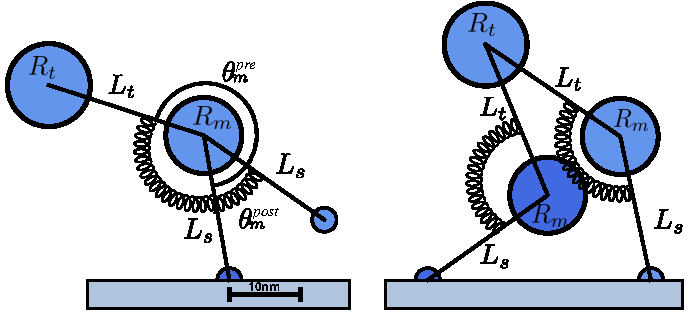
\includegraphics[width=1\linewidth]{figures/equilibrium-positions-final.pdf}
\caption{\textbf{Basic geometric model in pre-stroke and post-stroke states.}
 \textit{Left: } Pre-stroke model of dynein with one MTBD bound to microtubule and the other free. Angles are measured from the $+\hat{x}$ direction. \textit{Right: } Post-stroke model with both MTBDs bound to microtubule. MTBD angles are relative to $+\hat{x}$ direction, and motor angles are between stalk and tail. Lengths and radii not to scale.}
\label{fig:model}
\end{figure}

\begin{figure}[tbhp]
\centering
\includegraphics[width=0.5\linewidth]{../../plots/burgess-model-figure.pdf}%
%% \includegraphics[width=0.6\linewidth]{../../plots/grotjahn-model-figure.pdf}%
%% \includegraphics[width=0.3\linewidth]{../../plots/crystal-model-figure.pdf}%
\caption{\textbf{Scale model compared with experimental images.} \textit{Left:} Model with angles at pre-stroke equilibrium superimposed over axonemal dynein c heavy chain micrograph in the pre-stroke ADP-Vi-bound state \cite{burgess-paper}. Interdomain lengths and radii scaled to micrograph scale bar. No microtubule is present, so $\theta_{nb}$ is arbitrary. \textit{Right: } Model with angles at pre-stroke equilibrium superimposed over density map of full-length native cytoplasmic dynein with accessory tail proteins (map ID EMD-7000) \cite{grotjahn}. Interdomain lengths and radii scaled to density map.}
\label{fig:micrographs}
\end{figure}


%% Model at equilibrium angles superimposed over an axonemal dynein c micrograph consisting of an apo and and ADP-Pi-bound dynein monomer \cite{burgess-paper}; axonemal and cytoplasmic dynein have comparable size and architecture \cite{dynein-c-paper}. \textit{Right:} Model at equilibrium superimposed over full-length dimerized dynein bound to accessory proteins,  Left figure has a scale bar of 15nm, right 26.3nm between MTBD and AAA1 of motor domain.


\begin{table}
  \centering
  \begin{tabular}{lrrr}
    Param & Model & Experimental & Source \\
    \hline
    $L_s$ & $\ls$ nm & $21$ nm & \cite{Burgess2003, 3vkh-cite, carter-paper}\\
    $L_t$ & $\lt$ nm & $23$ nm & \cite{Burgess2003, 3vkh-cite, carter-paper}\\
    $\theta_b$ & $\eqb$ &  120 & \cite{leschziner} \\
    $\theta_m^{\mbox{pre}}$ & $\eqmpre$ &  197 & \cite{Burgess2003}\\
    $\theta_m^{\mbox{post}}$ & $\eqmpost$ & 242 & \cite{Burgess2003}\\
    $\theta_t$ & $\eqt$ &  & \\
    $R_t$ & $\radiust$ nm & $4$ nm & \cite{Burgess2003}\\
    $R_m$ & $\radiusm$ nm & $5.5$ nm & \cite{Burgess2003}\\
    $R_b$ & $\radiusb$ nm & $1.25$ nm & \cite{Burgess2003}\\
    \hline
  \end{tabular}
  \caption{Constant parameters used in simulation. $L_s$ and $L_t$ are the lengths of the stalk and tail interdomain linkers. The $\theta$ parameters are the equilibrium values for each angle, where $\theta_m^{\mbox{pre}}$ is the equilibrium angle for the unbound motor in pre-stroke, whereas $\theta_m^{\mbox{post}}$ is the equilibrium angle for the bound pre-stroke motor and both post-stroke motors. $R_b$, $R_m$ and $R_t$ are the MTBD, motor and tail radii. Parameters used for all simulations unless otherwise noted}
  \label{table:constparams}
\end{table}

\begin{table}
  \centering
  \begin{tabular}{lr}
    Param & Model  \\
    \hline
    $c_b$ & $\cb \Delta G_{ATP}$ \\
    $c_m$ & $\cm \Delta G_{ATP}$  \\
    $c_t$ & $\ct \Delta G_{ATP}$  \\
    $k_a$ & $\kstk$  $s^{-1}$  \\
    $k_b$ & $\kb$  nm $s^{-1}$  \\
    $\epsilon$ &  $\MTbindingdistance$ nm  \\
    $k_{ub}$ & $\kub$ $s^{-1}$  \\
    $C$ & $\cexp$  \\
    \hline
  \end{tabular}
  \caption{Free parameters used in simulation. $c_b$, $c_m$ and $c_t$ are the MTBD, motor and tail spring constants, respectively. $k_a$ is the affinity transition rate from high to low affinity when MTBD unbinds. $k_b$ and $k_{ub}$ are the rates of pre-stroke to post-stroke and post-stroke to pre-stroke transitions, respectively. $\epsilon$ is the vertical position allowed for rebinding. $C$ is the tension-gating factor.}
  \label{table:params}
\end{table}

\section*{Model}
This model is meant to capture the coarse-grained structural, dynamical and chemical properties of the full dynein complex, while remaining mathematically simple. The structural features of dynein are captured through a two-dimensional geometric model of circular domains connected by rigid rods, shown in Figure \ref{fig:model}. The dynamics of dynein are simulated by imposing both equilibrium and Brownian forces on each circular domain of the model. The chemical properties of dynein are emulated by sporadically transitioning the model between two states: a poststroke state where both binding domains are fixed to the microtubule, and a prestroke state where one foot is free to diffuse. This was influenced by similar simulations done before \cite{zhaomodel}. The poststroke state is meant to represent dynein after rebinding free MTBD and undergoing the motor-MTBD conformational change, but before releasing ADP, according to the Tsygankov scheme \cite{tsygankovscheme}. The prestroke state represents the dynein after binding ATP, unbinding from the MT and undergoing a motor conformational change, but before rebinding the MT. ATP hydrolysis and Pi rejection are ignored by the model. These two states were chosen because ADP release is thought to be the rate limiting step for the whole cycle \cite{holzbaur1989}, and the post-unbinding conformational change is expected to happen soon after MT unbinding \cite{mogamirate}, meaning the post-unbinding conformation should dominate when unbound from MT. We constrain our model to move through only the most likely mechanochemical cycle according to \textit{Tsygankov et al} \cite{tsygankovscheme}, where a head remains in the ADP-bound post-stroke state while the other head goes through the entire mechanochemical cycle, neglecting other possible cycles. Each state feels equilibrium forces on its domains meant to mimic the structural changes which occur during the cycle \cite{burgess-paper, burgessknight}. In particular, the equilibrium angles governing a tail-motor-MTBD angle change cause a displacement of the free MTBD towards the MT minus end, producing a forward step.

\subsubsection*{Model geometry}
The dynein model represents a full dynein complex consisting of two dynein heavy chains dimerized by a large tail domain. The model accounts for the following domains within the complex: two microtubule binding domains (``MTBD''), two AAA+ heptad motor domains, and a tail domain consisting of many dynein light chains and a dimerization site. MTBDs, motor domains and the tail are all represented by circles of radius $R_b$, $R_m$ and $R_t$, respectively. Each MTBD is connected to a motor domain via a rigid rod of length $L_s$, meant to represent the stalk domain. Each motor domain is connected to the tail domain via a rigid rod of length $L_t$; this rod represents the heavy chain linker and intermediate/light chains which connect the motor to the dimerization site.

Values for $R$ and $L$ were acquired by aligning the dynein model with EM micrographs of the full dynein complex \cite{burgess-paper,grotjahn}, as shown in Figure \ref{fig:micrographs}. See Table \ref{table:params} for these values. $L_t$, the stem length between motor domain and tail, was calculated as the distance between the center of the EM motor domains and identified dimerization site in the tail domain \cite{}. However, studies which compare truncated GST-linked dynein lacking a tail and native dynein find the two step with similar dynamics \cite{weihongpaper-i-think}, suggesting that our model with an $L_t$ value from native dynein should be comparable with studies on truncated dynein constructs as well.

\subsubsection*{Equilibrium forces}
The prestroke state has four degrees of freedom: $\theta_{bb}, \theta_{bm}, \theta_{um}$ and $\theta_{ub}$. The poststroke state has two: $\theta_{nm}$ and $\theta_{fm}$. The model is free to vary across all of these degrees of freedom, depending on its state, barring steric interactions with the microtubule. These angles describe a planar model which is not capable of transverse motion. To capture the gross dynamics and interdomain oscillations of the protein, restoring forces are imposed on each angle about equilibrium angles $\theta^{eq}_{bb}, \theta^{eq}_{bm}, \theta^{eq}_{um}, \theta^{eq}_{ub}$ for prestroke and $\theta^{eq}_{nm}$ and $\theta^{eq}_{fm}$ for poststroke. Each domain $i$ has a harmonic energy $c_i\left(\theta_i-\theta^{eq}_i\right)^2$ which exerts a restoring force pushing it back to equilibrium, where $c_b$, $c_m$ and $c_t$ are spring constants for each domain. These equilibrium angles are taken to be the average angle occupied by the protein in solution, and are thus extracted from EM micrographs, shown in Figure \ref{fig:micrographs}. These angles were extracted from axonemal dynein, but structural similarity suggests they should be applicable to cytoplasmic dynein as well \cite{dynein-c-paper}. Electron microscopy studies using ADP-Vi to freeze dynein in the pre-stroke state allow for both pre- and post-stroke equilibrium angles to be found \cite{burgess-paper}.

The rigid rod geometry and equilibrium angles can be used to calculate the mean step size. If all joints except the tail joint are treated as rigid, then two steps are possible: a forward step of $6.3$nm and a backwards step of $73$nm. This serves as a validation of the geometry of the model, which reproduces the experimental mean step size of XYZ \cite{xyz}.

\subsubsection*{Binding}
Conformational changes on nucleotide binding, also known as the mechanochemical cycle \cite{cianfrocco}, are captured by transitioning the model between the prestroke and poststroke states. During prestroke, the free MTBD must first release from the MT by transitioning from high to low affinity. The affinity transition rate, $k_a$, governs this process. Binding can then occur when the prestroke model's unbound foot diffuses near enough the microtubule. When within a distance of $\epsilon$, binding occurs at a rate of $k_b$ (Table \ref{table:params}). On binding, the prestroke model changes state to a poststroke model while retaining the positions of its domains. The previously unbound domain is transported to the microtubule.

\subsubsection*{Unbinding}
Unbinding occurs when a poststroke MTBD unbinds from the microtubule. This event can occur for either MTBD, and each domain has its own unbinding rate $k_{ub}$. To account for the tension-gating proposed by Yildiz \textit{et al} \cite{yildizcleary}, we bias forward directionality by influencing a MTBD to unbind based on the separation distance with the opposing MTBD. For domain $i \in \{n, f\}$ with binding domain angle $\theta_{ib}\left(\theta_{nm}, \theta_{fm}\right)$, unbinding rate is given by $\rho_{ub} = k_{ub}e^{-C\left(\theta_{ib}-\theta^{eq}_{ib}\right)}$, where $C$ is a parameter of the model. This will bias the model to unbind more preferentially for the lagging MTBD due to a higher likelihood for $\theta^{eq}_{ib} > \theta_{ib}$ for the lagging head. Values used for parameters $k_{ub}$ and $C$, along with $k_a$ and $k_b$, are shown in Table \ref{table:params}.

The transitions between prestroke and poststroke events in the mechanochemical cycle \cite{cianfrocco} are captured by changing the motor equilibrium angles when a state transition occurs. The prestroke state has an unbound motor angle closer to $\pi$ than the prestroke motor\cite{burgess-paper}; thus, on unbinding, the unbound MTBD should experience a restoring force effecting the post-to-pre conformational change. On rebinding, the motors transition back to the poststroke equilibrium, producing restoring forces causing the pre-to-post conformational change. This shifting of equilibria, coupled with alternating the freedom of the active MTBD, is meant to mimic the coupling of ATPase activity and MTBD affinity in the real dynein motor.

\subsubsection*{Brownian dynamics}
Brownian dynamics is used to study the model's dynamics in a biophysical manner. In the Brownian regime, protein motion is given by $\dot{\vec{X}} = \frac{1}{\gamma}\left(\vec{F}+\vec{R}\right)$. In the model, each circular domain has its own associated $\gamma$ factor given by Stokes' Law as $\gamma_i = 6\pi\nu R_i$ with dynamic viscosity $\nu$ \cite{stokeslaw}. The force on each domain is given by $\vec{F} = \vec{F}_{spr} + \vec{T}$, where $\vec{T}$ is the tension force between domains maintaining the rigid rod constraint. Each domain feels not only a harmonic restoring force, but also a Brownian force $\vec{R}$. This force is a Gaussian-distributed zero-mean magnitude with variance $R_{\sigma^2} = \sqrt{\frac{2k_bT\gamma}{\delta t}}$ and uniformly random direction.

\subsubsection*{Monte Carlo}
A Monte Carlo algorithm governs the simulation of the step. We initialize a two-headed bound configuration of dynein by randomly picking domain angles and calculating the total harmonic energy by summing the energies of each domain. A probability of unbinding, $P_{ub}$, is then calculated from a Boltzmann distribution, where $P_{ub}\propto e^{-\beta E_{total}}$ (\todo{is this right? we don't use just the binding angle?}). If dynein unbinds, then the configuration transitions into the one-headed bound state where Brownian dynamics is performed. This process is repeated to generate an ensemble of independent configurations which takes a single step and contributes to a large sample of stepping staistics. A partition function, $Z=\sum e^{-\beta E{total}}$, can then calculate ensemble averages of unbinding rates and probability. \todo{maybe a bit more info on how you go from binding to unbinding over the course of a single simulation, especially wrt L; readers may not know how this works}

%\section*{Fitting $k_b$ and $k_{ub}$}
%To fit the binding and unbinding rate constants $k_b$ and $k_{ub}$ a simple theoretical model for stepping was used, similar to one previously published \cite{myosindutyratio}. First, it is assumed that the unbinding rate of an MTBD does not depend on the binding state of the other MTBD, that is, that there is no inter-head coordination. Then the dissociation rate of the whole complex from the microtubule, $k_{dis}$, is estimated as $k_{dis} = P(ob)*k_{ub} = \frac{\bar{t}_{ob}}{\bar{t}_{step}} * \frac{1}{\bar{t}_{bb}}$, where $P(ob)$ is the probability of a dynein complex being in the prestroke state, $\bar{t}_{ob}$ and $\bar{t}_{bb}$ are the expected durations for a prestroke and poststroke state, and $\bar{t}_{step} = \bar{t}_{ob} + \bar{t}_{bb}$ is the expected step duration. Plugging in the last definition yields $k_{dis} = \frac{\bar{t}_{step} - \bar{t}_{bb}}{\bar{t}_{step}\bar{t}_{bb}}$. Introducing a new variable $\bar{t}_{run}$, the average run length of in vivo dynein, and using the relation $\bar{t}_{run} = k_{dis}^{-1}$, a new relation is found for poststroke time: $\bar{t}_{bb} = \frac{\bar{t}_{run}\bar{t}_{step}}{\bar{t}_{run}+\bar{t}_{step}}$. Using the definition of $\bar{t}_{step}$ a similar relation is found for prestroke time: $\bar{t}_{ob} = \frac{\bar{t}_{step}^2}{\bar{t}_{step}+\bar{t}_{run}}$. Finally, using the relation $\bar{t}_{step} = \frac{v}{L_{step}}$ for dynein velocity $v$ and expected tail step length $\bar{L}_{step}$, the following equations are found for prestroke and poststroke time in terms of experimental observables of velocity, run time and step length:
%
%  \begin{align}
%    \bar{t}_{ob} &= \frac{\bar{L}^2}{\bar{v}^2\left(\bar{L}/v+\bar{t}_{run}\right)}\\
%    \bar{t}_{bb} &= \frac{\bar{L}\bar{t}_{run}}{v\left(\bar{t}_{run}+\bar{L}/v\right)}
%  \end{align}
%
%  For estimating prestroke and poststroke times from Yildiz \textit{et al}\cite{yildiz}, a velocity of $124 nm/s$ is used. A study with a similar velocity is used to estimate $\bar{t}_{run} = 1060 nm / 134 nm / s = 7.9s$ \cite{weihongpaper}. These observables, along with $\bar{L} = 8nm$, yield estimations $\bar{t}_{ob} = 5.2*10^{-4}s$ and $\bar{t}_{bb} = 6.4 * 10^{-2}s$.

\subsubsection*{Prestroke motion equations derivation}
Brownian Dynamics was used to describe the motion of each domain, indexing with $i \in \{bb, bm, t, um, ub\}$, corresponding to bound-binding, bound-motor, tail, unbound-motor, unbound-binding:

  \begin{align}
    \dot{X_i} &= \frac{1}{\gamma_i}\left(F^x_i + R^x_i\right)\\
    \dot{Y_i} &= \frac{1}{\gamma_i}\left(F^y_i + R^y_i\right)
  \end{align}

  where $F^{x/y}_i$ is the force projection on coordinate $x/y$ of domain $i$, and $R^x_i$ the Brownian force, a Gaussian zero-mean force with variance $R_{\sigma^2} = \sqrt{\frac{2k_bT\gamma}{\delta t}}$ \cite{einstein}. Transforming position variables to polar coordinates results in four degrees of freedom: $\theta_{bb}, \theta_{bm}, \theta_{um} and \theta_{ub}$. Performing this transformation and expanding the force term yields the following equations:

  \begin{multline}
    \dot{X_i}\left(\theta_{bb}, ..., \theta_{ub}, \dot{\theta}_{bb}, ..., \dot{\theta}_{ub}\right) = \frac{1}{\gamma_i}\big(F^{spr}_x(\theta_{bb}, ..., \theta_{ub}) + \\
    \lambda_i\left(X_{i+1}-X_i\right) + \lambda_{i-1}\left(X_i-X_{i-1}\right)R^x_i\big)
    \label{eq:ob-system}
  \end{multline}

  \begin{multline}
    \dot{Y_i}\left(\theta_{bb}, ..., \theta_{ub}, \dot{\theta}_{bb}, ..., \dot{\theta}_{ub}\right) = \frac{1}{\gamma_i}\big(F^{spr}_y(\theta_{bb}, ..., \theta_{ub}) + \\
    \lambda_i\left(Y_{i+1}-Y_i\right) + \lambda_{i-1}\left(Y_i-Y_{i-1}\right)R^y_i\big)
    \label{eq:ob-system-other}
  \end{multline}

  where the $\lambda$ terms are tension terms needed to maintain the rigid rod constraints and $\vec{F}^{spr}$ the harmonic equilibrium forces felt by each domain. Each $X_i$ coordinate is related to the $\theta_j$ coordinates via the recursive formulas $X_{i>1} = L_i\cos(\theta_{i-1})+X_{i-1}$ and $Y_{i>1} = L_i\sin(\theta_{i-1})+Y_{i-1}$ for y-coords. Thus, each $\dot{X_i}$ term is linearly related to one or more $\dot{\theta_j}$ terms.

  There are $n$ unknown $\theta_j$ values and n unknown $\lambda$ values, totaling $2n$ unknown variables. There are $2n$ equations linear in $\dot{theta_j}$ and $\lambda_q$, $n$ each from the X and Y equations. The system of equations provided by Equation $\ref{eq:ob-system}$ was solved in Matlab, yielding equations for all $\dot{\theta_j}$.

\subsubsection*{Poststroke motion equations derivation}
Brownian dynamics was initially used for the postroke case but was later changed to be simulated with Monte Carlo methods. After running simulations undergoing Brownian dynamics for both states, we saw a large time spent in this poststroke state causing it to frequently reach equilibrium and be independent of our dynein's stepping pattern. We decided to shorten this process by simulating this state with Monte Carlo algorithms that sample from a Boltzmann distribution of the dynein's total energy. 
*Talk about choosing random configuration of dynein and calculating its total energy from each conformer. 
%% Brownian dynamics was also used for the poststroke case. Due to the added constraint of both binding domains being fixed to the microtubule, the model is fully described by angles $\theta_{nm}$ and $\theta_{fm}$; see Figure \ref{fig:model}. The positions of non-bound domains are defined by the following equation for $i \in \{nb, nm, t, fm, fb\}$, corresponding to near-binding, near-motor, tail, far-motor and far-binding domains:

%%  \begin{multline}
%%    \dot{X_{i\neq\{nb, fb\}}}\left(\theta_{nm},\theta_{fm}, \dot{\theta_{nm}}, \dot{\theta_{fm}}\right) = \frac{1}{\gamma_i}\big(F^{spr}_x(\theta_{nm}, \theta_{fm}) + \\
%%    \lambda_i\left(X_{i+1}-X_i\right) + \lambda_{i-1}\left(X_i-X_{i-1}\right) + R^x_i\big)
%%    \label{eq:bb-system}
%%  \end{multline}

%%  \begin{multline}
%%    \dot{Y_{i\neq\{nb, fb\}}}\left(\theta_{nm},\theta_{fm}, \dot{\theta_{nm}}, \dot{\theta_{fm}}\right) = \frac{1}{\gamma_i}\big(F^{spr}_y(\theta_{nm}, \theta_{fm}) + \\
%%    \lambda_i\left(Y_{i+1}-Y_i\right) + \lambda_{i-1}\left(Y_i-Y_{i-1}\right) + R^y_i\big)
%%    \label{eq:bb-system}
%%  \end{multline}

%%  Coordinate velocities are similarly linear with $\dot{\theta_{nm}}$ and $\dot{\theta_{fm}}$. This system has six independent equations and six unknowns $\dot{\theta_{nm}}, \dot{\theta_{fm}}, \lambda_{nb}, \lambda_{nm}, \lambda_{t}, \lambda_{fm}$. Analytic solutions were acquired using Mathematica.

\subsubsection*{Simulating the model}
Simulations began in the poststroke equilibrium state. The model was time-evolved via Euler's Method using analytic expressions for $\{\dot{\theta}_{bb}, \dot{\theta}_{bm}, \dot{\theta}_{um}, \dot{\theta}_{ub}\}$, using a timestep of $dt = 10^{-10}s$. In the prestroke state, during each timestep the model had a $k_b*dt$ probability of transitioning into the poststroke state, where $k_b = k_b^0\left(1-H\left(X_{uby}-0.1\right)\right)$, where H is the Heaviside function. On transition to poststroke, proper $\theta_{nm}$ and $\theta_{fm}$ angles and proper interhead separation $L$ were calculated to yield a poststroke model with identical cartesian positions to the old poststroke, except with the previously unbound binding domain moved to $y=0$. Once in poststroke, the model was time-evolved via Euler's Method using analytic expressions for $\{\dot{\theta}_{nm}$ and $\dot{\theta}_{fm}\}$ and a timestep of $dt=10^{-10}s$. Each timestep, the poststroke model had a $k_{ub}*dt$ chance of transitioning to prestroke, where $k_{ub} = k^0_{ub}e^{-c(\theta-\theta_{eq})}$. On transitioning, proper values of $\{\theta_{bb}, \theta_{bm}, \theta_{um}, \theta_{ub}\}$ were calculated to create a prestroke model with identical cartesian positions to the old poststroke model.

  %% \section*{Calculating leading/lagging probability vs displacement}

  %% \section*{Calculating force-dependent velocities}


\section*{Results}
Structural parameter lengths $L_t$, $L_s$ and radii $R_b$, $R_m$, and $R_s$ were estimated from crystal structures of cytoplasmic dynein \cite{3vkh-cite, carter-paper}. Motor domain equilibrium angles were estimated from EM class averages of axonemal dynein in the absence of neucleotide for the two-head-bound (2HB) angle or in the presence of irreversibly-binding ADP-Vi for the one-head-bound (1HB) angle \cite{Burgess2003}, shown in Figure \ref{fig:micrographs}. The binding equilibrium angle $\theta_b$ was estimated from a crystal structure of cytoplasmic dynein bound to tubulin \cite{leschziner}.

The other parameters shown in Table \ref{tab:params} were estimated by simulating the model and tuning parameters to experimental measurements, as described as follows. These single step Brownian dynamics simulations were run at a constant temperature of $T=310.15 K$  with an Euler's method time step of $dt = 10^{-13}$ $s$. The Monte Carlo algorithm simulated $>18000$ step cycles for each initial unsigned distance of $L_i \in [1, 72]$. The algorithm's fast computation allowed flexible optimization for each parameter in order to most accurately replicate stepping results from experiment. We investigated this parameter space by associating stepping parameters to experimental measurements of dynein's step. Results are shown for a model with parameters described in Table \ref{tab:params}.

Model springs were chosen to reproduce experimental step sizes. The model generated forward-directed motion with a mean step size of \forjin{what is the mean step size? I think David said somewhere he wanted us to note this - could potentially do the mean while ignoring the small steps?}, as shown in Figure \ref{fig:SteppingPlots}.b. The model takes steps in the range of $<-40nm$ to $>55nm$, encompassing the range observed for TIRF microscopy studies of cytoplasmic dynein \cite{}. The ratio of short to long steps is comparable for model and experiment. The large number of short ($<4nm$) steps the model takes comes from step events where the unbound head quickly rebinds after dissociating from the microtubule. We note that fluorescence-based measurements cannot resolve near zero-length steps, so it is impossible to compare experimental and model behavior in this range.

\begin{figure}[tbhp]
\centering
\begin{subfigure}{.75\columnwidth}
	\centering
	\includegraphics[width=1\linewidth]{../../plots/mc_plots/u_step_length_probability_distribution_2.5_5.50e+10_1.00e+08_0.0_1.0_1.0_120.0_197.0_242.0_-0.35}
\end{subfigure}
\begin{subfigure}{.2\columnwidth}
	\centering
	\includegraphics[width=1.3\linewidth]{../../plots/mc_plots/u_colorbar_2.5_5.50e+10_1.00e+08_0.0_1.0_1.0_120.0_197.0_242.0_-0.35}
\end{subfigure}
\includegraphics[width=1\linewidth]{../../plots/mc_plots/u_step_length_1d_probability_density_2.5_5.50e+10_1.00e+08_0.0_1.0_1.0_120.0_197.0_242.0_-0.35}
\caption[Stepping statistics of model]{\textbf{Stepping statistics of model.} \textit{Top: } Heatmap of initial foot displacement vs. step length. Initial displacement defined as position of the stepping MTBD minus the position of the stationary MTBD, before the step takes place. Step length defined as final displacement minus initial displacement. Linear regression calculated in orange, compared with Yildiz's linear regression plotted in red. Contours of 90\%, 50\%, 25\%, and 5\% displayed as white lines. \textit{Bottom: } Probability density of model step sizes plotted against Yildiz's distribution of step sizes. }
\label{fig:SteppingPlots}
\end{figure}

The interstep correlation, which we define as the correlation between the head separation of one step and the next, was mostly influenced by the dynamics of unbinding and rebinding of the stepping head. In order to best replicate experimental observation of interstep correlation, we optimized the binding parameters, $k_a$ and $k_b$, to allow for moderate interstep correlation. Figure \ref{fig:SteppingPlots} displays a heat map of initial displacement, defined as the signed distance from the stationary MTBD to the stepping MTBD, vs. the step length. Experimental data \cite{} measure dynein's interstep correlation at $m = -0.4$. The negative slope implies a bias for negative displacements to take forward steps while the positive displacements take negative steps. We fit $k_a$ and $k_b$ according to this slope and achieved $m = -0.492$ with values from Table \ref{table:params}. The binding parameters largely influenced the dependence between steps by influencing the rate for rebinding and controlling the tendency to equilibriate during the unbound state. More specifically, the affinity transition rate, $k_a$, controlled the transition time from high to low affinity when unbinding to introduce a buffer period and prevent instantaneous rebinding. The binding rate, $k_b$, controlled the tendency for the MTBD to rebind after being within $\epsilon$ of the MT. To achieve experimentally realistic correlations, both binding rates were increased significantly to promote quick and immediate rebinding after unbinding. Lower binding rates would allow the 1HB state to reach equilibrium and lose information about the previous step. The bottom figure in Figure \ref{fig:SteppingPlots} shows the probability density of step lengths compared to a stepping histogram from Yildiz \textit{et al.} experiment. The peak near 0 nm displays the effect of the large binding rates; the model preferred steps within -8 to 8 nm 56\% of the time. Despite the fast rebinding, the simulation was still able to achieve forward directionality with larger forward steps than negative ones.

%% The interstep correlation, which we define as the correlation between the head separation of one step and the next, was mostly influenced by the dynamics of unbinding and rebinding of the stepping head. If the constant governing unbound head rebinding, $k_b$, was too small then the unbound head would always equilibrate and there would be no correlation between steps. If $k_b$ was large then most model steps would be small the the model would be only weakly forward-directed. The affinity time $k_a$, which controls how long the unbound head can freely diffuse before rebinding, needed to be high enough to prevent instantaneous rebinding. With these parameters properly set, the model generated an interstep correlation of m=-0.492 as in Figure \ref{fig:SteppingPlots}.a, which accords with interstep correlations from experiments \cite{}.

%modifications from jins original: move some discussion stuff into the discussion, change the emphasis to results over choosing parameters

In addition to angular energy, the unbinding process is also governed by a factor $C$. Called the tension gating factor, $C$ controls how likely a lagging head is to unbind compared with a leading head. By tuning $C$, we managed to reproduce experimentally determined domain unbinding preference \cite{yildizpaper}, as shown in Figure \ref{fig:ProbLagPlot}.

In addition to angular energy, the unbinding process is also governed by a factor $C$. Called the tension gating factor, $C$ controls how likely a lagging head is to unbind compared with a leading head. We determined $C$ based on the experimental likelihood for a lagging head to unbind vs. the interhead separation \cite{yildizpaper}. A test for the lowest root-mean-squared error between the experiment and the model generated a value of $C=-0.35$, as shown in Figure \ref{fig:ProbLagPlot}. This parameter governs the tension-gating between dynein's heads, as the probability of a lagging step increases with $C$. Consequently, $C$ does not affect the dependence on the time spent in the 2-HB state 

\begin{figure}[tbhp]
	\centering
	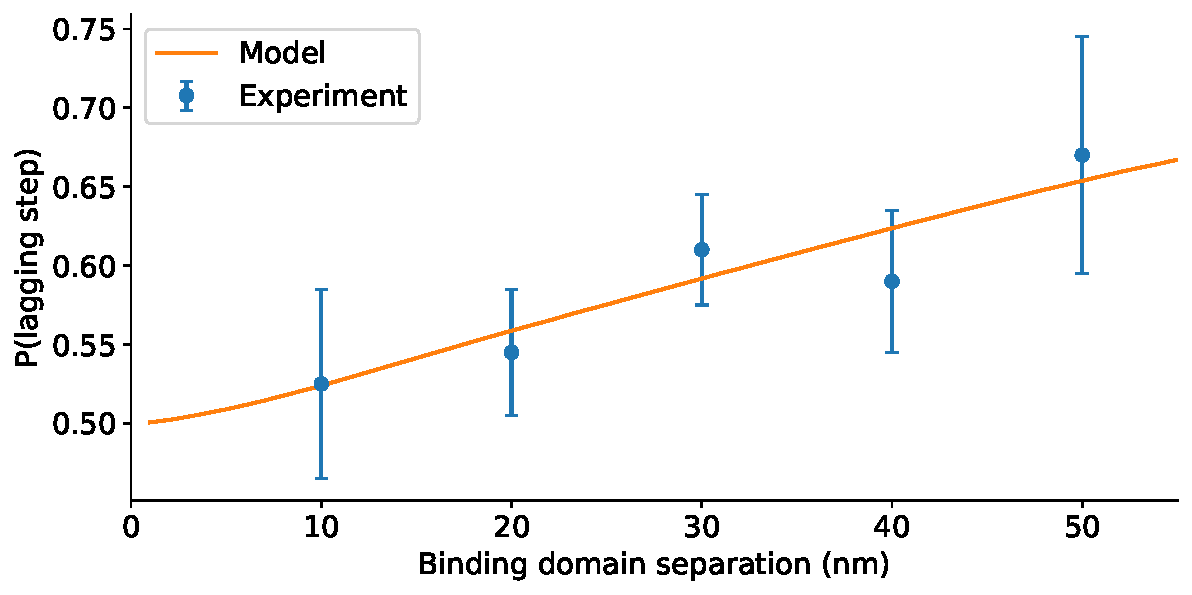
\includegraphics[width=\linewidth]{../../plots/mc_plots/prob_lagging_vs_init_L_-0.35}
	\caption[Lagging preferred steps]{\textbf{Lagging preferred steps.} Likelihood of a trailing step vs. the initial binding domain distance ($P_{trail.}(L)$. Exponential unbinding parameter, $C$, fitted with \cite{Dewitt2012}.}
	\label{fig:ProbLagPlot}
\end{figure}

%\subsection*{$k_{ub}$}
Dynein has been seen to spend most of its time in the both-heads-bound state \cite{}, and so the duration of this state almost completely determines dynein's velocity. The unbinding rate directly correlates to the rate of steps, as the inverse, $k_{ub}^{-1}$, is the average time spent in the 2-HB state. We tuned our unbinding rate $k_{ub}$ such that the model's velocity was 26 nm/s, comparable with experimentally observed velocities from TIRF microscopy \cite{yildizpaper}. When sequential steps are stitched together trajectories can be generated, as seen in Figure \ref{fig:TrajPlot}. We note that the unbinding parameter is specific to the experimental preparation, as the unbinding process is sensitive to ATP concentration \cite{}.

\begin{figure}[ht]
	\centering
	\includegraphics[width=\linewidth]{../../plots/mc_plots/u_trajectory_plot_2.5_5.50e+10_1.00e+08_0.0_1.0_1.0_120.0_197.0_242.0_-0.35}
	\caption[Stepping trace of head labeled dynein]{\textbf{Stepping trace of head labeled dynein.} Trajectory of MTBD over 24 seconds of walking. Red and blue labeled heads shows independence from each other during processive walking. Experimentalal trace from \cite{Dewitt2012} offset by 120 nm to display comparison. Average velocity of 26 nm/s for both traces.}
	\label{fig:TrajPlot}
\end{figure}

\newpage

%
%\begin{figure}[tbhp]
%\centering
%\includegraphics[width=\linewidth]{../../plots/mc_plots/u_ob_time_probability_density_2.0_5.50e+10_1.00e+08_0.0_1.0_1.0_120.0_197.0_242.0_-0.5}
%\caption{\textbf{Probability distribution plot of final displacement vs. initial displacement.} Dimentions: $nm^{-2}$ (Probability per area of box).}
%\label{fig:final_disp_prob}
%\end{figure}


%%%%% OLD RESULTS SECTION: %%%%%%
%Motion equations were derived for the pre-stroke and post-stroke states of the model. The model was simulated by starting in the equilibrium post-stroke position and using Euler's method to time-evolve the model, using a timestep of 1e-10 \textit{s}. The model was transitioned between post-stroke and pre-stroke states using unbinding and binding rates. Model parameters were estimated from various experimental results. Spring constants were chosen to fit the model stepping size to single-molecule head-labelled experiments\cite{yildizpaper}, as outlined in Figure S\ref{fig:supp-model-fit}. Model rate constants were fit to motor velocities from the same experiment, along with theoretical calculations for the prestroke and poststroke times outlined in the Methods section. The tension-gating parameter $c$ was fit to the leading/lagging unbinding likelihood versus interhead separation from the same experiment, as shown in Figure \ref{fig:tensiongating}. Thirty-two 5-second simulations were run, each initialized with a different random seed. Each simulation was forward directed, took both forward and backward steps, and displayed stepping dynamics similar to that seen in experiment.
%
%As seen in Figure \ref{fig:trajectory}, the model is highly variant in trajectory, but biased to moving in the $+\hat{x}$ direction, corresponding to the microtubule minus-end. When unbound the free MTBD diffuses both parallel and perpendicular to the microtubule, reaching up to 50 \textit{nm} above the track. Though the unbound MTBD freely approaches the microtubule, it does not always bind, as seen in the $7-9 \mu s$ part of the simulation. The cartoons in Figure \ref{fig:trajectory} reveal the model taking on many conformations, revealing the model's structural flexibility. The model seems to prefer alternating hand-over-hand stepping, but occasionally takes steps in a semi-inchworm fashion, as seen at time $5.3 \mu s$ in Figure \ref{fig:trajectory}.

%\begin{figure}[tbhp]
%\centering
%\includegraphics[width=\linewidth]{../../plots/paper_trajectory_plot.pdf}
%\caption{\textbf{Model achieves forward-directed processivity.} \textit{Top view:} x-position of near and far binding domains during a 10 $\mu s$ simulation at high kinetic parameters of $k_b = \trajectorykb s^{-1}$ and $k_{ub} = \trajectorykub s^{-1}$. \textit{Middle view:} Cartoon snapshot of model at time indicated by bound binding domain. Teal lines correspond to the microtubule. \textit{Bottom view:} y-projection. Arrows on top and bottom plots correspond to respective snapshot times.}
%\label{fig:trajectory}
%\end{figure}

%The model was then compared to TIRF studies of dynein stepping in DeWitt \textit{et. al.} \cite{yildizpaper}. Figure \ref{fig:behavior}.a shows 8 representative model trajectories compared to experimental dynein. The eight simulations track experimental very well over 5 seconds, and average to the same position. The eight simulations end up distributed over a 200 \textit{nm} area, showing the variation in the model stepping extends to a variation in velocity in the long term. The step size distribution for the 32 simulations are shown in Figure \ref{fig:behavior}.b). The model is capable of taking both positive and negative steps, with steps extending from -40 \textit{nm} to 50 \textit{nm}, matching experimental dynein. The most probable step is 12 \textit{nm}, with an average step size of 6.2 \textit{nm}. This matches the peak experimental step size window of 7-13 \textit{nm}. The pre-stroke and post-stroke state occupation times are shown in Figure \ref{fig:behavior}.c and d.). The model prefers long pre-stroke times, but is capable of taking very fast steps. The post-stroke time has a heavy-tailed distribution. Experimental technique does not resolve time spent in pre- and post-stroke, but we outline a technique for calculating these values for experimental trajectories in Methods. These theoretical values correspond well to model behavior, and square with experimental findings that dynein is almost always in the post-stroke state \cite{imaiburgess}.

%\begin{figure}[tbhp]
%  \centering
%  \includegraphics[width=\linewidth]{../../plots/paper_model_behavior}
%\caption{\textbf{Stepping dynamics of model.} \textit{Top: } Average position of near and far MTBDs over 5 seconds of simulation and 8 random seeds. Trajectory compared with single-motor-labelled cytoplasmic dynein from DeWitt \textit{et. al.} \cite{yildizpaper}. \textit{Middle: } Model step size distribution from 32 5 second simulations. Step length is defined as the change in an MTBD position during a full step cycle. Also plotted is the head step size distribution from DeWitt \textit{et. al.} \cite{yildizpaper}. \textit{Bottom left: } Distribution of time spent in the pre-stroke state during a full mechanochemical cycle from the same dataset. \textit{Bottom right: } Time in the post-stroke state. Both bottom plots have the theoretical values for pre-stroke and post-powerstoke times from the DeWitt \textit{et. al.} stepping trajectory.}
%\label{fig:behavior}
%\end{figure}

%Dependence of the unbinding MTBD on its relation to its partner MTBD is studied in Figure \ref{fig:tensiongating}. Figure \ref{fig:tensiongating}.a shows a heat map of initial displacement, defined as how much the stepping MTBD is ahead of the stationary MTBD, vs the step size. A line of best fit is constructed with intercept $b=5.7$ and slope $m=-1$. This indicates a negative trend where large positive displacements are likely to cause backwards steps, and negative displacements are likely to cause forward steps. This is consistent with the idea of tension gating, where tension between the two motor heads drives unbinding to relieve tension. The negative trend is reproduced in DeWitt \textit{et. al}, which shows a slope of $m=-0.4$. Figure \ref{fig:tensiongating}.b shows the unbinding probability of the lagging head with distance to the leading head. As the distance becomes greater the lagging head is more and more likely to unbind, again consistent with tension gating. This trend also very closely tracks DeWitt \textit{et. al}.

%\begin{figure}[tbhp]
%  \includegraphics[width=\linewidth]{../../plots/paper_displacement_vs_step_length.pdf}
%  \includegraphics[width=\linewidth]{../../plots/paper_unbinding_probability_vs_displacement.pdf}
%  \caption{\textbf{Analysis of foot order on unbinding.} \textit{Top: } Heatmap of initial foot position vs length of ensuing step. Initial displacement defined as position of the stepping MTBD minus the position of the stationary MTBD, before the step takes place. Line of best fit calculated with equation shown in legend in orange. Line of best fit from the same plot in DeWitt \textit{et al} \cite{yildizpaper} on cytoplasmic dynein shown in blue. \textit{Bottom: } Likelihood of a lagging-MTBD unbinding event vs the absolute value of initial displacement for model. The lagging-MTBD is the MTBD with more negative x position. Probability calculated as P(lagging step)$ = k_{ub}^{\text{lag}} / \left(k_{ub}^{\text{lag}} + k_{ub}^{\text{lead}}\right)$, where $k_{ub}^{\text{lag}}$ is the lagging-MTBD unbinding rate and $k_{ub}^{\text{lead}}$ the leading-MTBD unbinding rate. Lagging step probability also shown for DeWitt \textit{et. al.} cytoplasmic dynein.}
%  \label{fig:tensiongating}
%\end{figure}
%
%The effect of force on the model was then assessed by applying an artificial force on the tail domain of the model in the $+\hat{x}$ direction. The results of this study are shown in Figure \ref{fig:force}. An expected decrease in velocity is seen as stronger and stronger negative forces are applied to the model, pulling it against its natural walking direction. Unlike experiment, a reversal in velocity is not seen for this trial, indicating that perhaps the dynamics of force-mediated velocity reversal are more complicated than what this simplified model can handle. The results are consistent with an experiment done by Grotjahn \textit{et. al} where force is applied via optical tweezers to dynein constructs and their velocity is assayed. It will need to be studied why odd behavior is seen in the mdoel for positive forces.

%\begin{figure}[tbhp]
%  \centering
%  \includegraphics[width=\linewidth]{../../plots/paper_force_vs_velocity.pdf}
%\caption{\textbf{Impact of force on model velocity.} Model response to force in the $+\hat{x}$ direction applied to tail domain. Velocity calculated using displacement after 2 seconds of simulation at standard parameters. Behavior compared with a similar experiment on a cytoplasmic dynein construct using optical tweezers from Gennerich \textit{et. al.} \cite{responsetoload}.}
%\label{fig:force}
%\end{figure}

%The independence of dynein steps is then studied in Figure \ref{fig:independence}. Whether dynein works like a Markovian process, where each step is a history-free, is an interesting question. Figure \ref{fig:independence} demonstrates the impact of initial displacement of MTBDs to their final displacement, before and after a step is taken. The asymmetry in the plot is indicative that the initial configuration of the motor does have significant impact on the later state. The Brownian forces act to mitigate momentum and prevent information transfer through motion. However, the binding orientation of the dynein model to the microtubule is stable through time, and can influence the binding orientation of dynein to the microtubule at a later time. There seems to be a roughly tension-gated process occurring where negative displacements initially lead to positive displacements later.

%\begin{figure}[tbhp]
%  \centering
%  \includegraphics[width=\linewidth]{../../plots/paper_initial_vs_final_displacement.pdf}\\
%  \includegraphics[width=\linewidth]{../../plots/paper_stacked_displacement_histogram.pdf}
%  \caption{\textbf{Analysis of stepping independence.} \textbf{a.)} Heatmap of MTBD displacement before and after a stepping cycle. Displacement defined as the unbinding MTBD's x coordinate minus the stationary MTBD's x coordinate, calculated before and after the step. Structure in the heat map suggests steps are not independent, but rather that correlation exists between starting position and step size. \textbf{b.)} Compound histogram of final displacement for different ranges of initial displacement.}
%\label{fig:independence}
%\end{figure}

%\begin{figure}[tbhp]
%  \centering
%  \begin{subfigure}[]{0.8\columnwidth}\caption{}\vspace{5pt}\includegraphics[width=\columnwidth]{figures/winch-powerstroke-cartoon}\end{subfigure}\vspace{10pt}\\
%  \begin{subfigure}[]{0.5\columnwidth}\caption{}\includegraphics[width=\columnwidth]{../../plots/bothbound_stroke_angles_bd}\end{subfigure}%
%  \begin{subfigure}[]{0.5\columnwidth}\caption{}\includegraphics[width=\columnwidth]{../../plots/bothbound_stroke_angles_md}\end{subfigure}\\
%  \begin{subfigure}[]{0.5\columnwidth}\caption{}\includegraphics[width=\columnwidth]{../../plots/bothbound_stroke_tailx_positions}\end{subfigure}%
%  \begin{subfigure}[]{0.5\columnwidth}\caption{}\includegraphics[width=\columnwidth]{../../plots/bothbound_stroke_taily_positions}\end{subfigure}\\
%  \begin{subfigure}[]{0.5\columnwidth}\caption{}\includegraphics[width=\columnwidth]{../../plots/bothbound_long_stroke_angles_bd}\end{subfigure}
%  \caption{\textbf{Dynein model exhibits powerstroke, not winch, dynamics.} \textit{A. left: } Schematic of winch model for dynamics during conformation changes associated with right monomer binding. On free MTBD binding, linker swing in the just-bound head pulls the tail and cargo in the direction of the just-bound MTBD. \textit{A. right: } Schematic of the powerstroke model for dynamics during during conformation changes associated with right monomer binding. On free MTBD binding, linker swing pushes the just-bound head and tail domains towards the minus-end of the MT and alters the just-bound stalk domain's angle with the MT. Subfigures b-e describe dynamics for the right monomer during post-binding conformation change; only data for steps with a positive step size is shown. \textit{b.) } Just-bound MTBD stalk angle relative to MT axis as a function of time since MTBD binding along with MTBD angle equilibrium (blue dotted line). \textit{c.) } Just-bound head angle, along with prestroke equilibrium (red dotted line) and poststroke equilibrium (blue dotted line). \textit{d.) } Change in tail domain x coordinate since MTBD binding. \textit{e.) } Value of tail domain y coordinate. All values sampled every $10 ns$. \textit{f.) } Just-bound MTBD stalk angle for the millisecond after binding, sampled every 20 $\mu s$. All values plotted as mean $\pm$ SD.}
%\label{fig:stroke}
%\end{figure}

%%%%%%%%%%%%%% DISCUSSION ABOUT MODELS: %%%%%%%%%%
%We then examined how the model took its forward steps. Two existing theories for motion generation are depicted in Figure \ref{fig:stroke}.a. The winch model \cite{carterwinch, uenoem, sarlahmodel, nicastro, kinoshitaPSwinch, lippert}, on the left, predicts that the prestroke to poststroke transition causes the just-bound motor's head to act like a winch, pulling the tail domain down and forwards toward the microtubule. The powerstroke model \cite{mallikps, burgessknight, robertspowerstroke, burgess-paper}, on the right, predicts that the transition will cause a lever-like action of the just bound stalk, pulling the just bound motor's head and tail forward. The most notable differences between these two models are whether the stalk angle changes during the stroke \cite{lippert}, and whether the tail domain moves closer or further from the microtubule. Arrows indicate these predictions in Figure \ref{fig:stroke}.a.
%
%The average change of motor angles and positions during the prestroke-to-poststroke transition is shown in subfigures \ref{fig:stroke}.b-e. Only positive steps were used for clarity. Subfigure \ref{fig:stroke}.b indicates the model's just-bound stalk experiences a consistent angular displacement after binding, rotating to point more towards the minus end of the MT. Interestingly, this transition takes the binding angle out of equilibrium. This transition is permanent once made, as shown in \ref{fig:stroke}.f, which shows the no change even up to a millisecond after binding. This forward transition of the head domain is accompanied by a forward displacement of the tail domain by roughly 12 $nm$, as shown in Figure \ref{fig:stroke}.d, and a displacement away from the microtubule by 5-8 $nm$, as shown in Figure \ref{fig:stroke}.e. This tail displacement takes roughly 300ns, which corresponds roughly to the prestroke-to-powerstroke transition time from MD \cite{mdstroke} (DOES IT ACTUALLY THOUGH? LOOK AGAIN). The motor angle is shown in Figure \ref{fig:stroke}.c to transition from the pre-stroke equilibrium to the post-stroke equilibrium in time with the stalk angle change. Taken together, this data indicates that our simulated dynein moves through a powerstroke-, not a winch-type mechanism. We hypothesize that the out of equilibrium state of the motor angle post-transition is highly energetic, and it is quicker for the model to re-equilibrate the high-energy state through pushing the motor forward in a powerstroke than winching the faraway bulky tail downwards.

%% \begin{figure*}[tbhp]
%%     \includegraphics[width=0.5\linewidth]{../../plots/paper_foot_order_histogram.pdf}
%% \caption{The left plot is the $C=0$ case where the unbinding rate is
%%   independent of angle.  Here ``alternating'' means that the binding
%%   domain which did not move last time moved this time.  Passing means
%%   that the moving foot was behind, and ended up in front.}
%% \label{fig:steppingorder}
%% \end{figure*}

\section*{Discussion ideas}
\begin{enumerate}
    \item something about our kb ka interplay
    \item is it interesting that we don't have stalk elasticity at all and managed to reproduce dynein's dynamics? there was that one paper (find paper) that mentioned that maybe stalk elasticity is super important; maybe this would be a good to mention in the intro as an example of an idea we think is wrong, stalk elasticity is not -necessary- for dynein's walk
\end{enumerate}

\section*{Discussion}
In this study we aimed to answer the question of whether dynein's structure, elastic properties, and mechanochemical cycle-induced conformational changes are sufficient to explain the motor's stepping dynamics. We modeled dynein as five circular domains representing two microtobule binding domain (MTBD) heads, two motor domains, and a tail domain, connected via rigid rods. Angular spring forces were added to the motor and binding domain joints to represent interdomain elasticity, and tension forces were imposed to maintain the rigid rod constraints. The mechanochemical cycle was represented in the model as two states: a two-head-bound (2HB) state where both binding domains were constrained to the microtubule, representing the poststroke state, and a one-head-bound (1HB) state where one MTBD is free to diffuse, representing the porestroke state. The conformational changes in the linker which occur during the powerstroke were represented by changing the equilibrium angle in the motor joint of the unbound dimer, resulting in a forward kick of the MTBD head. The diffusive search of the 1HB state was simulated using Brownian dynamics, and the 2HB state was simulated using a Monte Carlo algorithm for efficiency.

To determine how well this model reproduced dynein's stepping dynamics, we first needed to assess how realistically the model generated single steps. We found that by tuning the models spring constants it could generate the proper range of both forward and backward steps, and with the proper ratio of short to medium to long steps as well as negative steps, indicating our Brownian kinetic model successfully captured the rough dynamics of the single step process. From fitting we found that relatively loose tail and MTBD spring constants and a stiff motor domain produced the best stepping histogram; this agrees with another simulation which found tail and MTBD flexibility is necessary for large steps \cite{tsygankovemsimulation}.

We further imposed a tension gating mechanism to bias the motor towards lagging steps; however, this was insufficient to guarantee interstep correlations, since the mechanism only controlled which foot unbound, not how it diffused. We needed further tuning to reproduce the interstep correlation.

To assure gross timescale accuracy in addition to spatial accuracy, we tuned the unbinding rate of the model such that our velocity matched experiment.

Proper interstep correlation was achieved by tuning the binding rate governing the transition from 1HB to 2HB. An exponential rebinding block process prevented instantaneous rebinding of the free MTBD to the microtubule to allow it to diffuse. With the proper binding rate our model produced an m=-0.492 interstep correlation, consistent with experimental measurements of m=-0.4 \cite{}.

We note that there was a strong dependence of interstep correlation on the binding time constant. Small binding constants allowed the unbound MTBD to reach equilibrium, erasing information from the previous step. Large binding constans only allowed very quick steps. It is thus a prediction from our findings that dynein's stepping should be highly dependent on MTBD-MT affinity, and that experimentally lowering affinity through mutagenesis should destroy or reduce dynein's interstep correlation.

Another interesting finding is that in our model the mean single step is slightly shorter than the experimental 16nm step \cite{find-citation}. This suggests that perhaps the motor requires a diffusive search along the microtubule to find the next binding site. Alternatively, as has been recently demonstrated, perhaps an electrostatic mechanism is used to guide the MTBD to the next binding site using long-range interactions \cite{longrangemt}.

The model also displays both inchworm and hand-over-hand stepping, as in real dynein \cite{weihongpaper}

Our theoretical work draws upon and extends several past models \cite{sarlahmodel, trottmodel, tsygankovemsimulation, zhaomodel}. This paper's approach of using Brownian dynamics to realistically predict the diffusion dynamics of a structural model of dynein is a useful technique for testing mechanistic theories for biological feasibility and sufficiency, and to our knowledge is the first model to combine imaging and kinetics data with Brownian dynamics to quantify the influences of drag on the dynein motor. We believe that taking into account diffusion dynamics and drag is necessary to understand dynein's dynamics. However, our model neglects many features which may be important for real dynein's walk. For example, some have proposed that stalk flexibility is an important aspect of dynein's mechanism \cite{mdstalk, lippert, find-that-other-possibly-burgess-paper}. Other features like microtubule electrostatic interactions \cite{longrangemt}, binding angle dependent MTBD binding \cite{responsetoload} - ACTUALLY LOOK AT PAPER THOUGH, inter-head coordination \cite{tsygankovscheme, tsygankovemsimulation}, stalk flexibility???, Y and Z are also neglected. Although our work successfully demonstrates the sufficiency of our minimal set of assumptions for generating motion, a more biologically realistic model would need to take these listed features into account.


\bibliographystyle{unsrt}
\bibliography{paper}

\end{document}
